\documentclass[10pt, a4paper]{article}
    \usepackage[utf8]{inputenc}
    %\usepackage[english, spanish]{babel}
    %\usepackage{fullpage} % changes the margin
    \usepackage{graphicx} 
    \usepackage{enumitem} 
    \usepackage{chngcntr}
    \counterwithin{figure}{section}
    \renewcommand{\thesection}{\arabic{section}} 
    \renewcommand{\thesubsection}{\thesection.\arabic{subsection}}
    \renewcommand{\baselinestretch}{1.5}

    \usepackage{amsmath}
    \usepackage{mathptmx}
    \usepackage[spanish, es-tabla]{babel} %es-tabla añadido
    \usepackage{amssymb}
    \usepackage{makeidx}
    \usepackage{float}
    \pagenumbering{arabic}
    \usepackage[left=25mm, right=25mm, top=25mm, bottom=25mm]{geometry}

    \usepackage[backend=biber]{biblatex}
    \bibliography{referencias}

\begin{document}

    \begin{titlepage}
        \centering
        {\scshape\Large Universidad Central de Venezuela \par}
        {\scshape\Large Facultad de ingeniería \par}
        {\scshape\Large Escuela de ingeniería Eléctrica \par}
        {\scshape\Large Departamento de Electrónica, Computación y Control \par}

        \vspace{6cm}
        {\Large\bfseries Pre-Laboratorio 4 : Amplificador BJT\par}
        \vspace{5cm}

        \vfill
        \begin{flushright}
            Estudiante:\par
            Santana Ricardo C.I.:29571461 \par
            \vspace{1cm}  
        \end{flushright}
        \vfill
        {\large \today \par}
    \end{titlepage}

    \section{Introducción}

    Entre las diversas aplicaciones que tiene el transistor BJT cabe señalar su uso como amplificador, que al estudiar su comportamiento en un circuito sencillo, se pueden observar características y funcionalidades que pueden conformar un circuito mucho más complejo.
    
    Para operar como amplificador, un transistor debe estar polarizado en la región activa. El problema de polarización es el de establecer una corriente cd constante en el emisor (o el colector) que debe ser predecible e insensible a variaciones en temperatura, valor de $h_{FE}$, etc. Por tanto se analizará un circuito básico de amplificador que maneje corrientes bajas en la rama mencionada, de manera que esté en la zona activa.

    Por otra parte es importante estudiar la ganancia del circuito, que relaciona los voltajes de entrada con los de salida del amplificador, buscando que sea tan estable como la corriente de polarización del colector.
    
    Todos los datos recopilados permitirán establecer un modelo lineal de amplificador para elaborar y diseñar circuitos más complejos, con varias etapas de amplificación u otros procesos requeridos para lo que se desee implementar.

    \newpage

    \section{Objetivos}

    \subsection{Objetivo General}
    \begin{itemize}
        \item Estudiar el comportamiento dinámico de un amplificador básico de tensión, configuración emisor común.
    \end{itemize}

    \subsection{Objetivos Específicos}
    \begin{itemize}
        \item Familiarizar al estudiante con los parámetros dinámicos más importantes del BJT.
        \item Obtener experimentalmente las características más importantes de un amplificador básico de tensión como son: la ganancia de tensión, impedancia de entrada e impedancia de salida.
        \item Analizar el efecto sobre la ganancia de tensión en una configuración emisor común, al colocar una carga al amplificador.
        \item Analizar el efecto sobre la ganancia de tensión en una configuración emisor común, al colocar un condensador de desacoplo en paralelo con la resistencia de Emisor, primeramente sin carga en el amplificador y luego con carga.
    \end{itemize}

    \newpage

    \section{Marco Teórico}

    En la práctica, el estudio de amplificadores exige previamente un análisis en continua para determinar la polarización de los transistores. Posteriormente, es preciso abordar los cálculos de amplificación e impedancias utilizando modelos de pequeña señal con objeto de establecer un circuito equivalente. Ambas fases en principio son independientes pero están íntimamente relacionadas.

    \begin{figure}[h!]
        \centering
        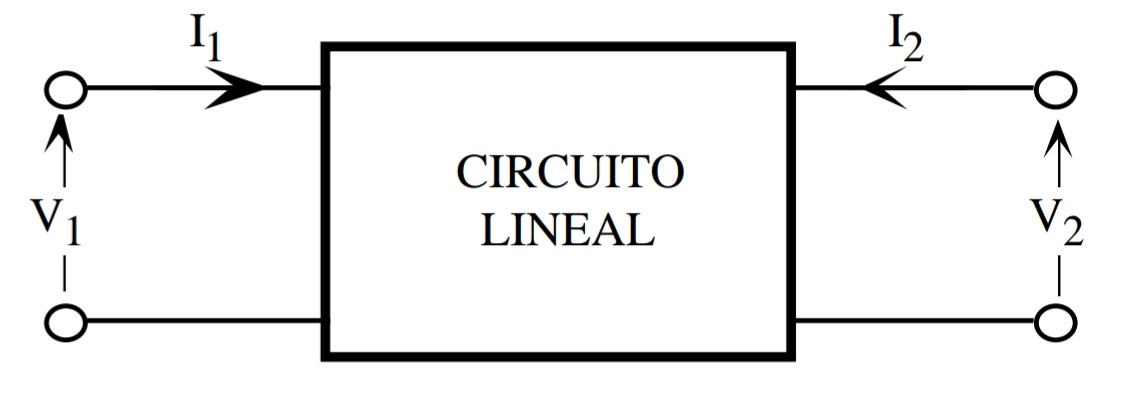
\includegraphics[height=4cm\textwidth]{circuito-lineal.jpg}
        \caption{Red bi-puerta}
        \label{fig:cir-lin}
    \end{figure}

    \subsection{Teoría de redes bipuerta}

    El comportamiento de un circuito lineal bi-puerta, tal como se muestra en la figura \ref{fig:cir-lin}, puede ser especificado a través de dos corrientes $(I_1, I_2)$ y dos tensiones $(V_1, V_2)$. En función de las dos posibles variables seleccionadas como independientes, ese circuito lineal puede ser caracterizado mediante cuatro tipo de parámetros ({Z}, {Y}, {H}, {G}), que en notación matricial, se expresan de la siguiente manera

    \begin{array}{c c}
        \begin{bmatrix}
            V_1 \\ 
            V_2 \\
        \end{bmatrix} = 
        \begin{bmatrix}
            z_i & z_r \\
            z_f & z_o
        \end{bmatrix}
        \begin{bmatrix}
            I_1 \\
            I_2
        \end{bmatrix} & 
        \begin{bmatrix}
            I_1 \\
            I_2 \\
        \end{bmatrix} = 
        \begin{bmatrix}
            y_i & y_r \\
            y_f & y_o
        \end{bmatrix}
        \begin{bmatrix}
            V_1 \\ 
            V_2 \\
        \end{bmatrix} \\

        \begin{bmatrix}
            V_1 \\ 
            I_2 \\
        \end{bmatrix} = 
        \begin{bmatrix}
            h_i & h_r \\
            h_f & h_o
        \end{bmatrix}
        \begin{bmatrix}
            I_1 \\
            V_2
        \end{bmatrix} & 
        \begin{bmatrix}
            I_1 \\
            V_2 \\
        \end{bmatrix} = 
        \begin{bmatrix}
            g_i & g_r \\
            g_f & g_o
        \end{bmatrix}
        \begin{bmatrix}
            V_1 \\ 
            I_2 \\
        \end{bmatrix} \\
    \end{array}
    
    Los parámetros {H} o h o híbridos son los que mejor caracterizan el comportamiento lineal de pequeña señal de un transistor bipolar. Estos parámetros relacionan la $V_1$ e $I_2$ con la $I_1$ y $V_2$ mediante la siguiente ecuación
    
    \begin{equation*}
        \begin{split}
            V_1 & = h_iI_1 + h_rV_2 \\
            I_2 & = h_fI_1 + h_oV_2 \\
        \end{split}
    \end{equation*}

    donde

    [W] $h_i = \frac{V_1}{I_1}\|_{V_2 = 0}$ = resistencia de entrada con salida en cortocircuito.

    [NO] $h_r = \frac{V_1}{V_2}\|_{I_1 = 0}$ = ganancia inversa de tensi n con entrada en circuito abierto

    [NO] $h_f = \frac{I_2}{I_1}\|_{V_2 = 0}$ = ganancia de corriente con salida en cortocircuito

    [$W^{-1}$] $h_o = \frac{V_1}{V_2}\|_{I_1 = 0}$ = conduc tan cia de salida con entrada en circuito abierto

    El modelo circuital en parámetros h de un circuito lineal se indica en la figura \ref{fig:h}.


    \begin{figure}[h!]
        \centering
        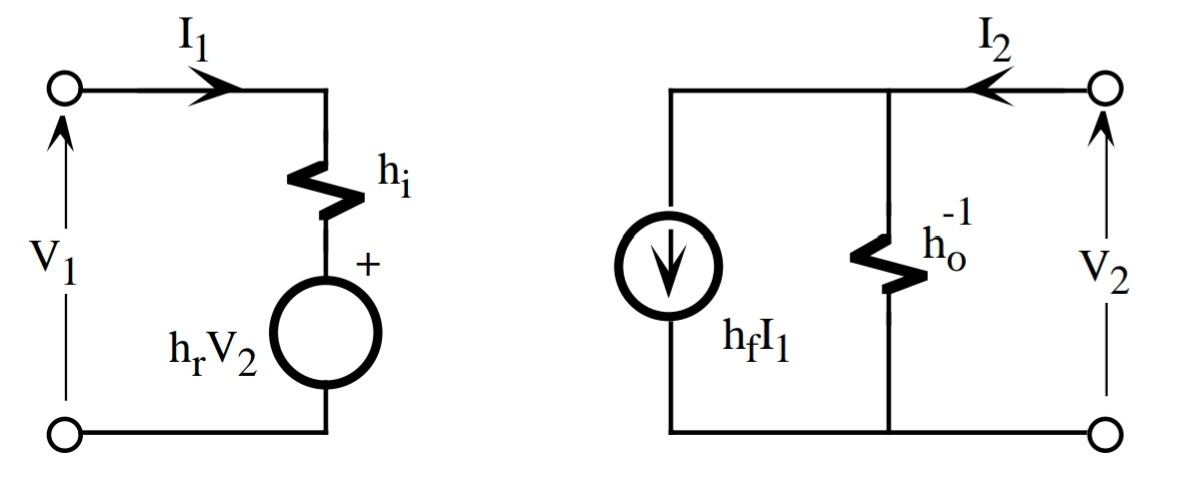
\includegraphics[height=4cm\textwidth]{parametrosh.jpg}
        \caption{Modelo equivalente en parámetros h.}
        \label{fig:h}
    \end{figure}

    \subsection{Análisis de un circuito empleando parámetros {H}}

    Un circuito lineal, por ejemplo un transistor actuando como amplificador, puede ser analizado estudiando su comportamiento cuando se excita con una fuente de señal externa VS con una impedancia interna RS y se añade una carga ZL, tal como se indica en la figura \ref{fig:amp-bas}. El circuito lineal puede ser sustituido por su modelo equivalente en parámetros {H} (figura \ref{fig:h}) resultando el circuito de la figura \ref{fig:amp-bas-h}. Existen cuatro parámetros importantes que van a caracterizar completamente el circuito completo: ganancia en corriente, impedancia de entrada, ganancia en tensión e impedancia de salida.

    \begin{figure}[h!]
        \centering
        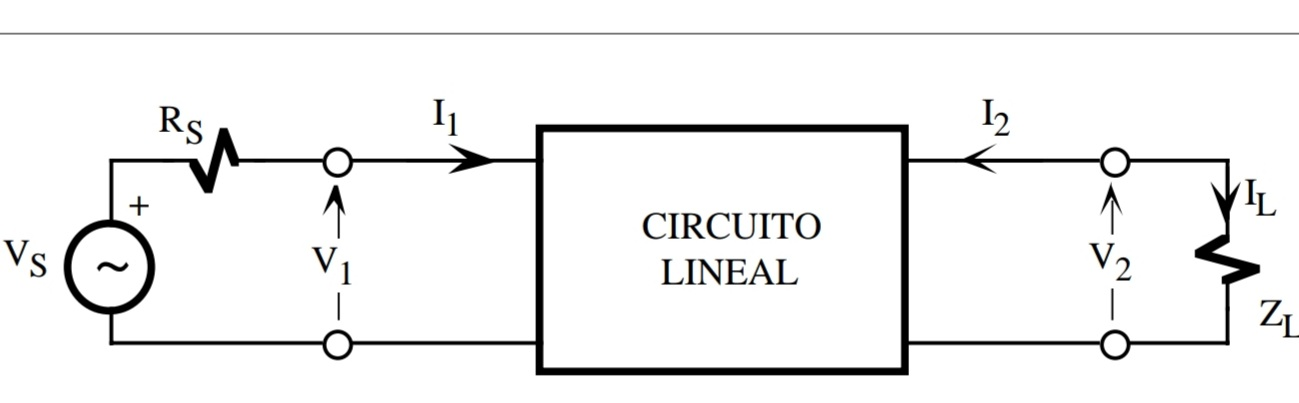
\includegraphics[height=4cm\textwidth]{amp-bas.jpg}
        \caption{Estructura de un amplificador básico}
        \label{fig:amp-bas}
    \end{figure}

    \begin{figure}[h!]
        \centering
        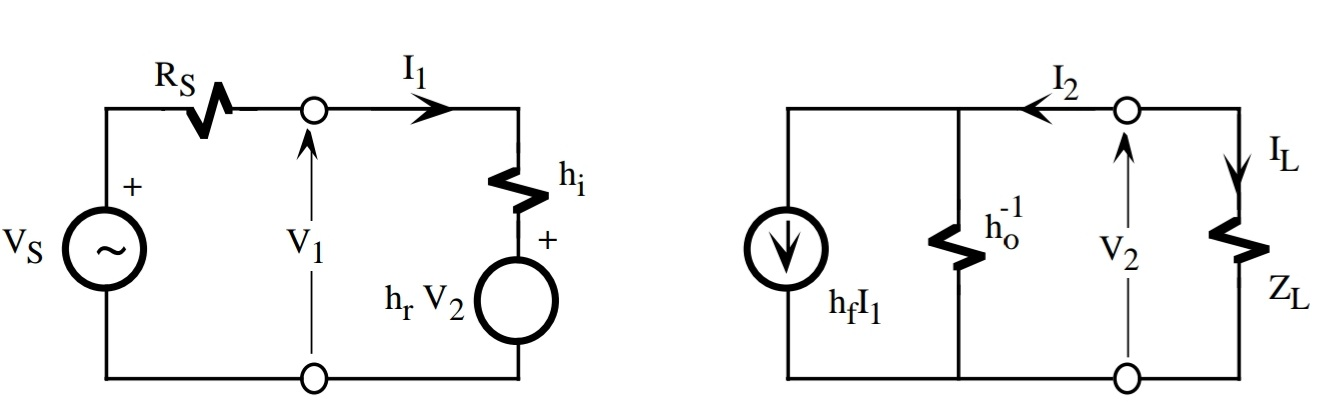
\includegraphics[height=4cm\textwidth]{amp-bas-h.jpg}
        \caption{Anterior circuito utilizando el modelo en parámetros h}
        \label{fig:amp-bas-h}
    \end{figure}

    \underline{\bf Ganancia de corriente.} Se define la ganancia de corriente de un circuito, AI, como la relación entre la intensidad de salida e intensidad de entrada, es decir,

    $$A_I = {I_L \over I_1} = -{I_2 \over I_1}$$

    Este cociente se obtiene resolviendo las siguientes ecuaciones extraidas del circuito de la figura \ref{fig:amp-bas-h},

    \left \{ \begin{equation*} %pendiente
        \begin{split}
            I_2 & = h_fI_1 + h_oV_2 \\
            V_2 & = -I_2Z_L 
        \end{split}
    \end{equation*} \right.

    Despejando, se obtiene que

    $$A_I = -{I_2 \over I_1} = -\frac{h_f}{1 + h_oZ_L}$$

    \underline{\bf Impedancia de entrada.} Se define la impedancia de entrada del circuito, $Z_i$, como la relación entre la tensión y corriente de entrada. Resolviendo el circuito de entrada se demuestra que

    $$Z_i = {V_1 \over I_1} = h_i + h_rA_IZ_L = h_i + \frac{h_fh_r}{{1 \over Z_L} + h_o}$$

    Nótese que la impedancia de entrada depende de la carga $Z_L$.

    \underline{\bf Ganancia de tensión.}  Se define la ganancia en tensión, AV, como la relación entre la tensión de salida y la tensión de entrada. Como se demuestra a continuación, la AV se puede expresar en función de la AI y la Zi, de forma que

    \begin{equation}
        A_v = {V_2 \over V_1} = {V_2 \over I_2}{I_2 \over I_1}{I_1 \over V_1} = -{V_2 \over I_L}{I_2 \over I_1}{I_1 \over V_1} = Z_LA_I{1 \over Z_i} = A_I{Z_L \over Z_i}
        \label{ganancia}
    \end{equation}

    \underline{\bf Impedancia de salida.} Se define la impedancia de salida, $Z_o$, vista a través del nudo de salida del circuito lineal como la relación entre la tensión de salida y la corriente de salida, supuesto anulado el generador de entrada y en ausencia de carga $(Z_L = \infty)$. Se demuestra que

    $$Z_o = {V_2 \over I_2}|_{V_S = 0, R_L = \infty} = \frac{1}{h_o - {h_fh_r \over R_S + h_i}}$$

    Estos cuatro parámetros permiten definir dos modelos simplificados muy utilizados en al análisis de amplificadores: modelo equivalente en tensión y modelo equivalente en intensidad. El modelo equivalente en tensión (figura \ref{fig:mod-ten}) utiliza el equivalente Thèvenin en la salida y el de intensidad (figura \ref{fig:mod-int}) el Norton. Ambos modelos son equivalentes y están relacionados por la ecuación \ref{ganancia}.

    \begin{figure}[h!]
        \centering
        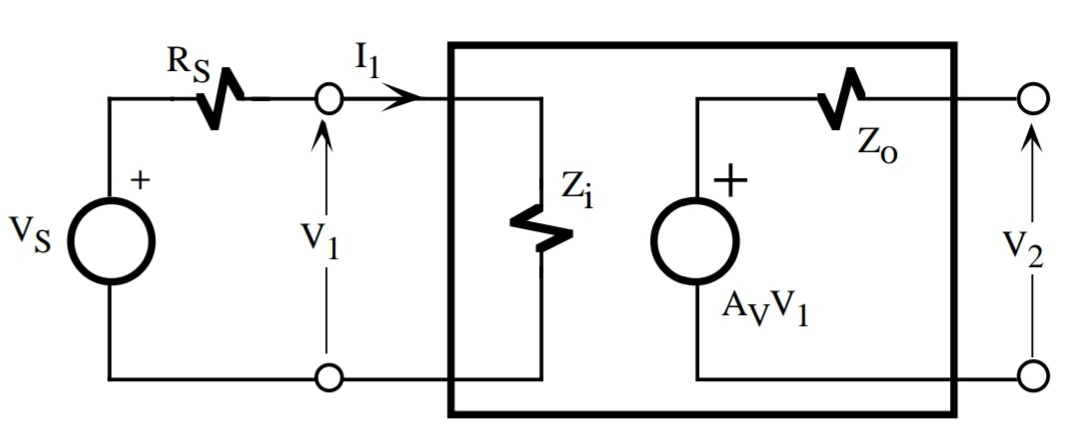
\includegraphics[height=4cm\textwidth]{mod-ten.jpg}
        \caption{Modelo equivalente en tensión}
        \label{fig:mod-ten}
    \end{figure}

    \begin{figure}[h!]
        \centering
        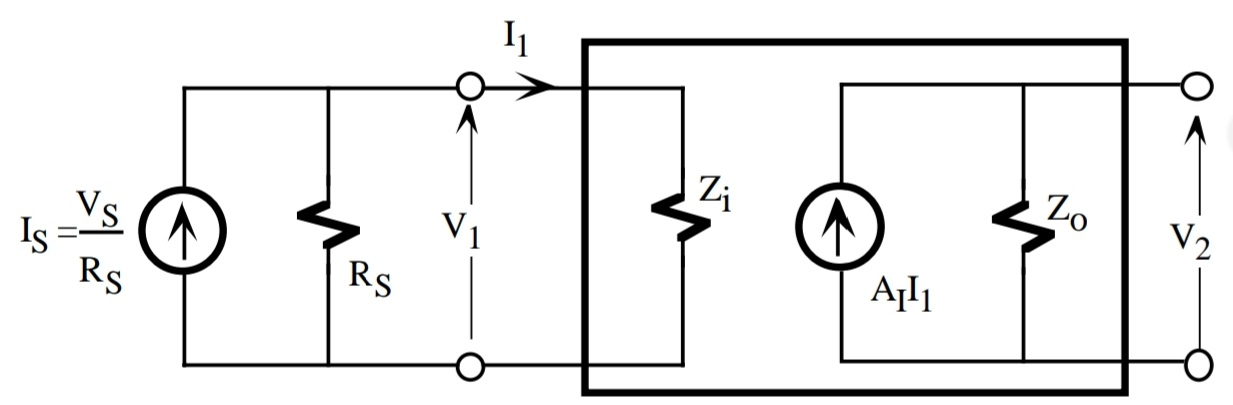
\includegraphics[height=4cm\textwidth]{mod-int.jpg}
        \caption{Modelo equivalente en intensidad}
        \label{fig:mod-int}
    \end{figure}

    La resistencia $R_S$ de la fuente de entrada influye en las expresiones de las ganancias de tensión o intensidad cuando se refieren a la fuente de excitación de entrada. En la figura \ref{fig:mod-ten}, la ganancia de tensión referida a la fuente $V_S$, $A_{VS}$, se obtiene analizando el divisor de tensión de la entrada formado por $R_S$ y $Z_i$, resultando

    $$A_{VS} = {V_2 \over V_S} = {V_2 \over V_1}{V_1 \over V_S} = A_V \frac{Z_i}{Z_i + R_S}$$

    De la misma manera, la ganancia de intensidad referida a la fuente IS (figura \ref{fig:mod-int}), $A_IS$, se obtiene analizando el divisor de corriente de entrada formado por $R_S$ y $Z_i$, resultando

    $$A_{IS} = {I_L \over I_S} = {I_L \over I_1}{I_1 \over I_S} = A_I \frac{R_S}{Z_i + R_S}$$

    Despejando en de la últimas dos ecuaciones $A_V$ y $A_I$, y sustituyendo en \ref{ganancia}, se obtiene la relación entre $A_{VS}$ y $A_{IS}$, dando como resultado

    $$A_{VS} = A_{IS}{Z_L \over R_S}$$

    \newpage

    \section{Metodología}

    \subsection{Trabajo Previo al Laboratorio}

    La estructura básica amplificadora corresponde al circuito de la Figura \ref{fig:circuito} sin RL y CE. Para éste circuito realice lo siguiente:

    \begin{figure}[h!]
        \centering
        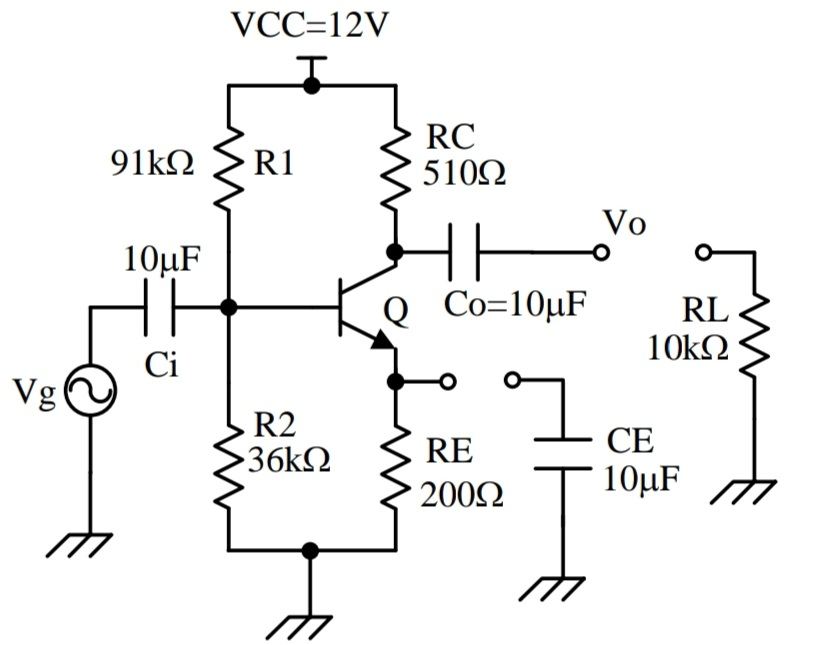
\includegraphics[height=4cm\textwidth]{amplificadorbjt.jpg}
        \caption{Amplificador Básico BJT}
        \label{fig:circuito}
    \end{figure}

    \begin{enumerate}
        \item Determine el punto estático de operación. \label{p1}
        \item[label=p2] Calcule utilizando los parámetros híbridos del transistor, la ganancia de tensión $A_V$, impedancia de entrada $Z_{in}$ y la impedancia de salida $Z_o$. \label{p2} %pendiente p2
        \item Coloque la resistencia de carga RL y repita el punto 1\ref{p2}.
        \item Sin RL, coloque un condensador paralelo a la resistencia RE y repita el punto \ref{p2}.
        \item Con RL y CE repita el punto \ref{p2}.
    \end{enumerate}

    \subsection{Trabajo de Laboratorio}

    \begin{enumerate}
        \item Para el circuito de la Figura \ref{fig:circuito}, sin el generador de entrada (Vg), los condensadores (Ci, Co y CE) y la carga RL, mida la tensión en el Colector ($V_C$), tensión en la Base ($V_B$) y la tensión en el Emisor ($V_E$) para determinar el punto estático de operación en el informe.
        \item \underline{Amplificador básico de la Figura \ref{fig:circuito} sin RL y CE.}
        \begin{enumerate}
            \item Coloque en el generador una señal senoidal de frecuencia 1kHz, promedio nulo y amplitud 2Vp-p. Conecte los condensadores Ci, Co y el generador de entrada (Vg).\label{p21}
            \item Con el osciloscopio en DC, observe y dibuje la señal en el Colector del transistor. Mida la amplitud pico-pico, la tensión pico máxima y el nivel DC de la onda. \label{p22}
            \item Con el osciloscopio en AC en ambos canales y en doble canal. Observe y dibuje la onda de la entrada (Vg) y la salida (Vo). Mida la frecuencia y amplitud pico-pico de las ondas para luego determinar la ganancia de tensión Av en el informe.
            \item Mida experimentalmente los valores de tensiones para luego determinar en el informe las impedancias de entrada y de salida del amplificador.
            \item Suba la amplitud de la señal de entrada hasta el punto donde comienza a distorsionarse la señal de salida. Mida la amplitud pico-pico de la señal de salida y de entrada. Dibuje ambas formas de onda.
            \item Suba hasta el máximo la amplitud de la señal de entrada y mida ésta amplitud pico-pico. Dibuje las ondas. \label{p26}
        \end{enumerate}
        \item \underline{Amplificador básico de la Figura \ref{fig:circuito} con RL y sin CE.}
        \begin{enumerate}
            \item Con las mismas condiciones colocadas en el punto \ref{p21}, repita los puntos \ref{p22} hasta \ref{p26}.
        \end{enumerate}
        \item \underline{Amplificador básico de la Figura \ref{fig:circuito} sin RL y con CE.}
        \begin{enumerate}
            \item Con las mismas condiciones colocadas en el punto \ref{p21}, repita los puntos \ref{p22} hasta \ref{p26}.
        \end{enumerate}
        \item \underline{Amplificador básico de la Figura \ref{fig:circuito} con RL y con CE.}
        \begin{enumerate}
            \item Con las mismas condiciones colocadas en el punto \ref{p21}, repita los puntos \ref{p22} hasta \ref{p26}.
        \end{enumerate}
    \end{enumerate}

    \newpage

    \section{Cálculos prévios}

    Se trabajará con el transistor npn PN2222A, el cual posee las siguientes especificaciones:

    %modelo tabla
    %\begin{table}[t]
        %probar con \centering
    %    \begin{center}
    %        \begin{tabular}{| r | l |}
    %            Fruta & Cantidad \\ \hline
    %            Manzana & 4 \\
    %            Naranja & 10 \\
    %            Plátano & 3 \\ \hline
    %        \end{tabular}
    %        \caption{fruta disponible} %nombre de la tabla
    %        \label{tab:fruta} %indice de la tabla
    %    \end{center}
    %\end{table}
    
    \begin{table}[h!]
        \centering
        \caption{Características del transistor PN2222A} %nombre de la tabla
        \label{tab:especificaciones} %indice de la tabla
        \begin{tabular}{c}
            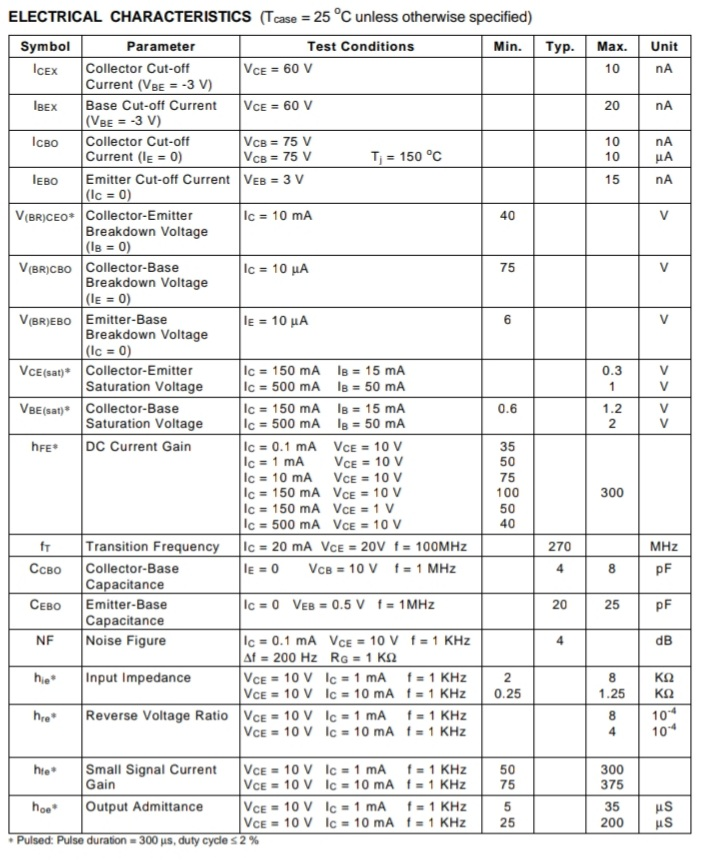
\includegraphics[height=20cm\textwidth]{pn2222a.jpg} \\
        \end{tabular}
    \end{table}
    
    de las cuales se deduce que:
    $\beta = h_{FE} = 150 \; @ \; I_C = 10mA; \; V_{CE} = 10V$
    $V_{BEsat} = 0.7V \; @ \; I_C = 150mA; \; I_B = 10mA$
    $h_{ie} = 5K\Omega \; @ \; I_C = 1mA; \; V_{CE} = 10V; \; f = 1KHz$
    $h_{fe} = 175 \; @ \; I_C = 1mA; \; V_{CE} = 10V; \; f = 1KHz$

    %\setcounter{equation}{1}
    %\begin{equation}
    %    \label{eq2}
    %    V_{CE} = V_{CC} - R_C\beta I_B - R_E(\beta + 1)I_B
    %\end{equation}

    Se determina el punto estático de operacion basandose en el circuito de la Figura \ref{fig:1}

    \begin{figure}[h!]
        \centering
        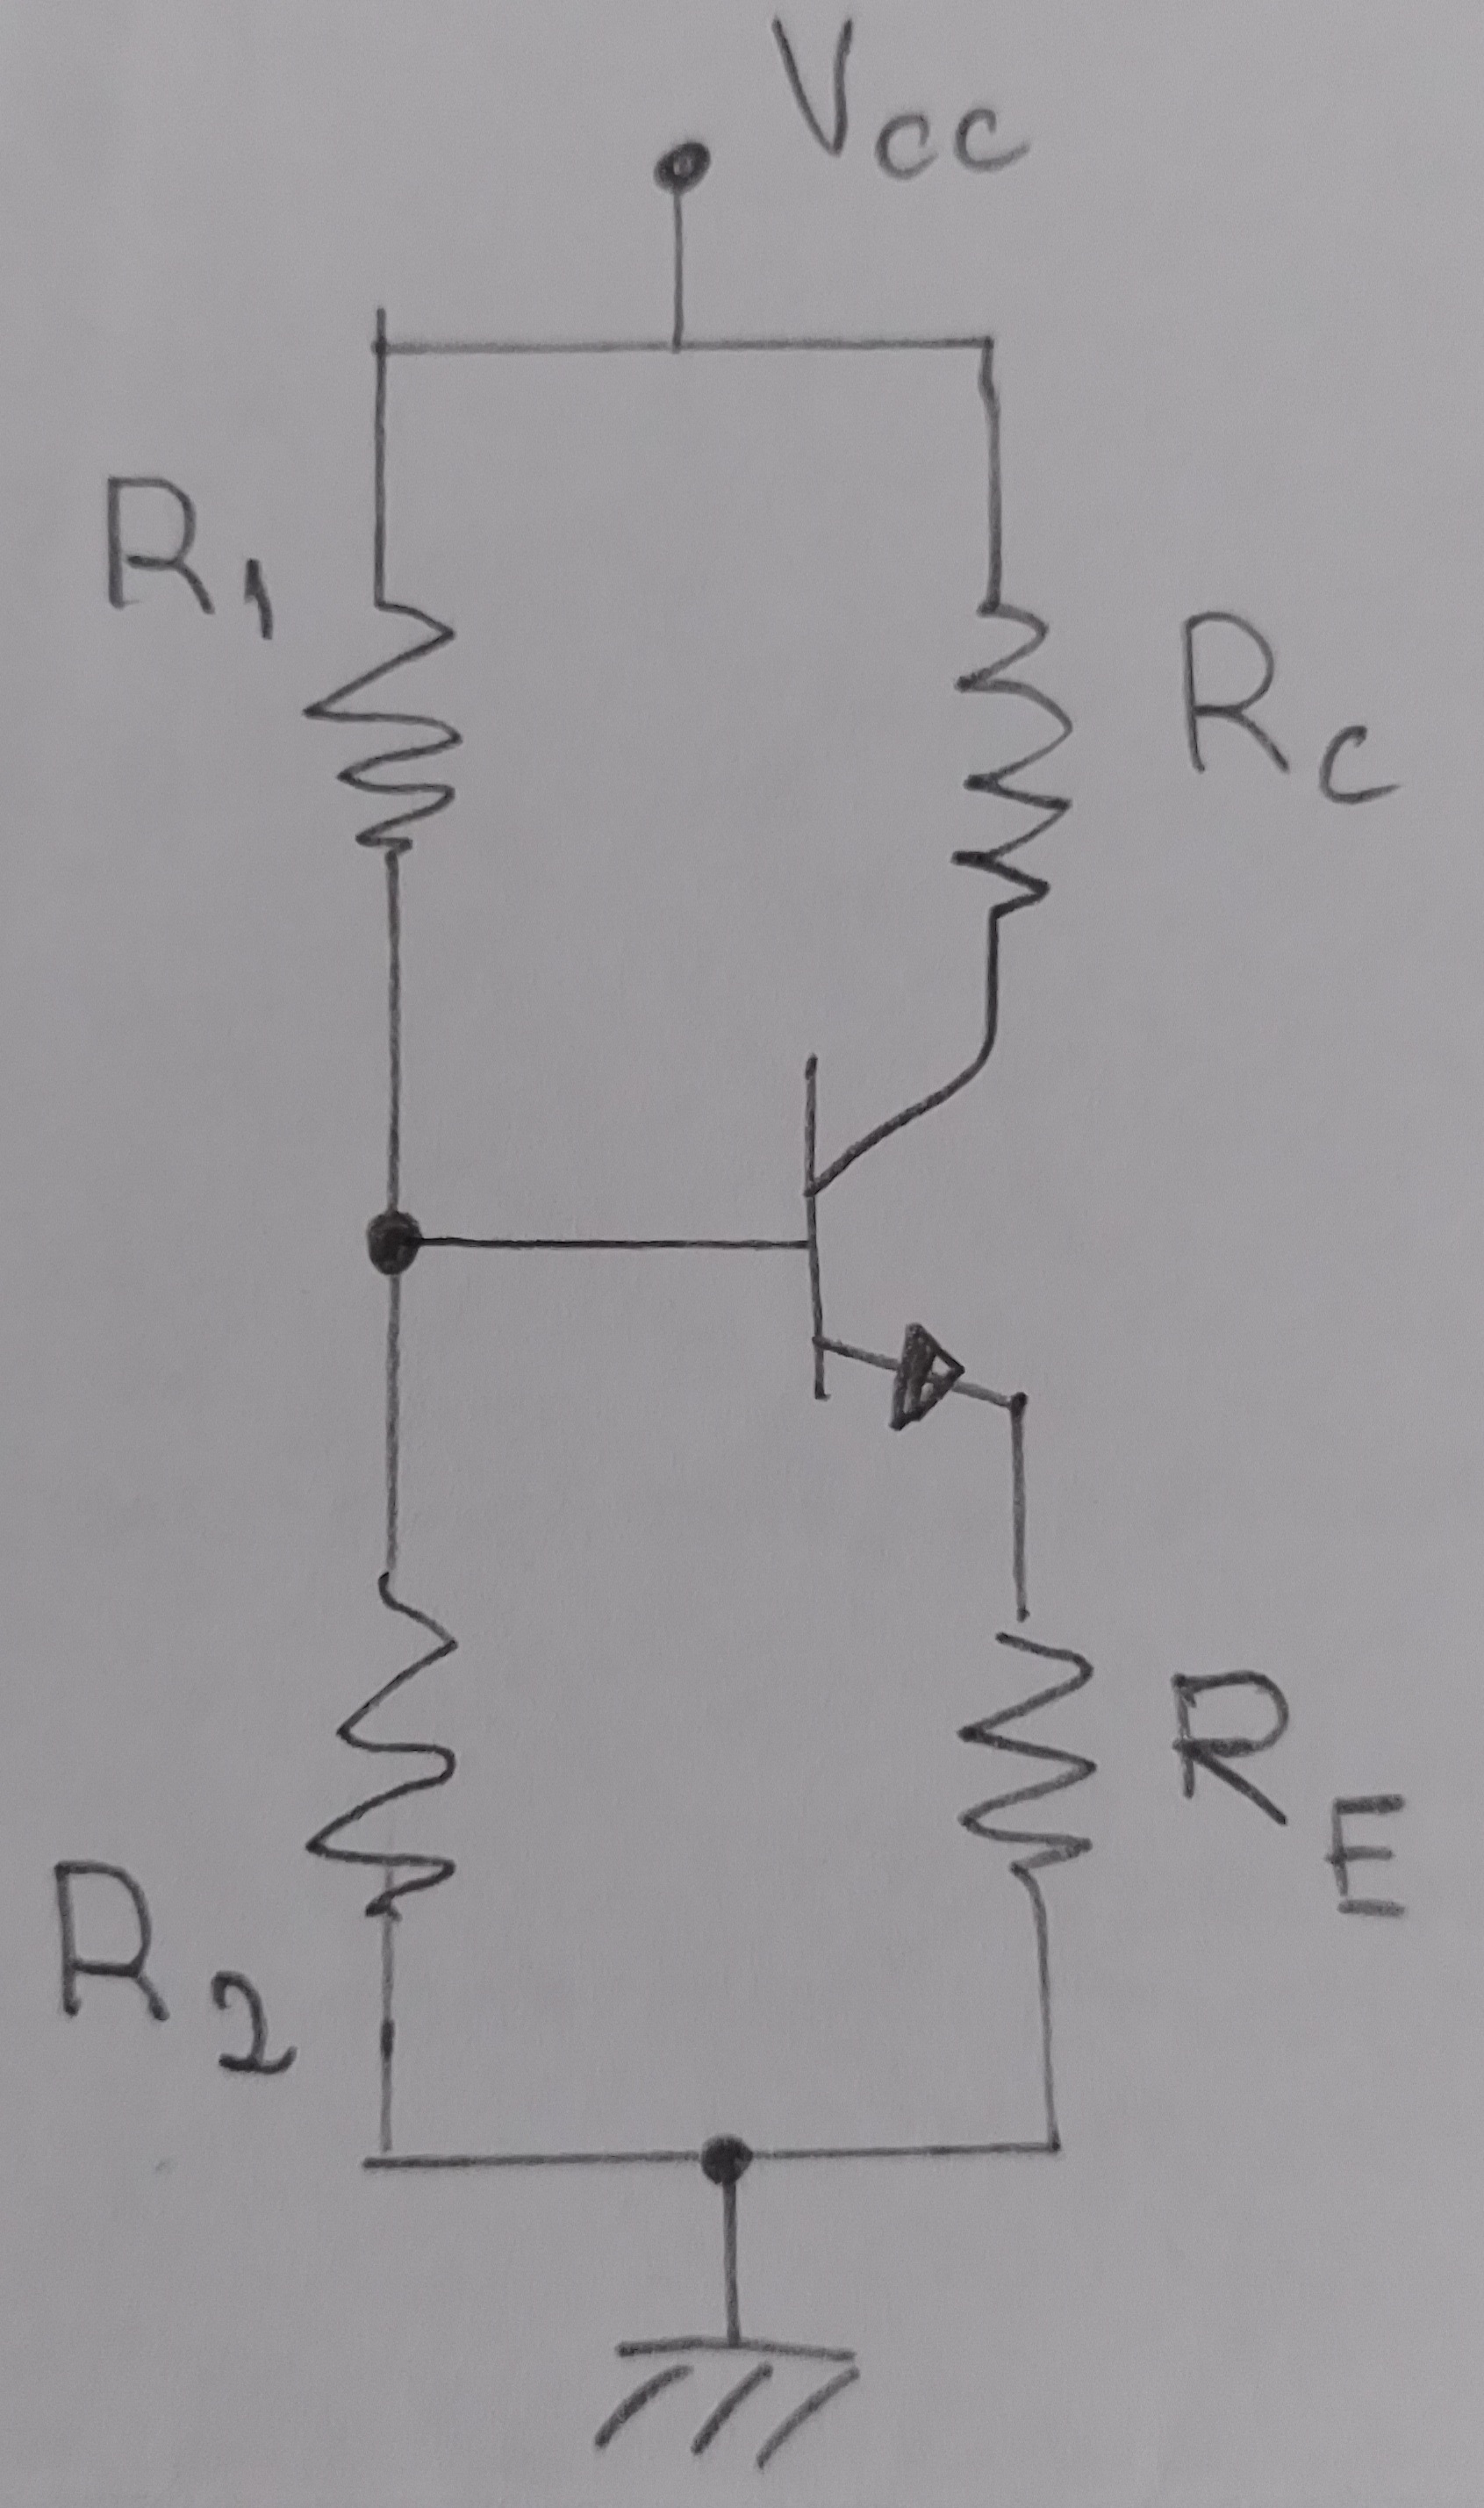
\includegraphics[height=4cm\textwidth]{qestatico.jpg}
        \caption{Circuito de operación estática}
        \label{fig:1}
    \end{figure}

    Calculando equivalente de thevelin entre la base del transistor y la referencia
    
    \begin{split}
        R_{Th} & = R_1 || R_2 = \frac{R_1R_2}{R_1 + R_2} \\
        R_{Th} & = \frac{(91K\Omega)(36K\Omega)}{91K\Omega + 36K\Omega} = 25.8K\Omega
    \end{split}
    
    por divisor de voltaje

    \begin{split}
        V_{Th} & = \frac{R_2}{R_1 + R_2} V_{CC} \\
        V_{Th} & = \frac{36K\Omega}{91K\Omega + 36K\Omega} (12V) = 3.4V
    \end{split}

    \begin{figure}[h!]
        \centering
        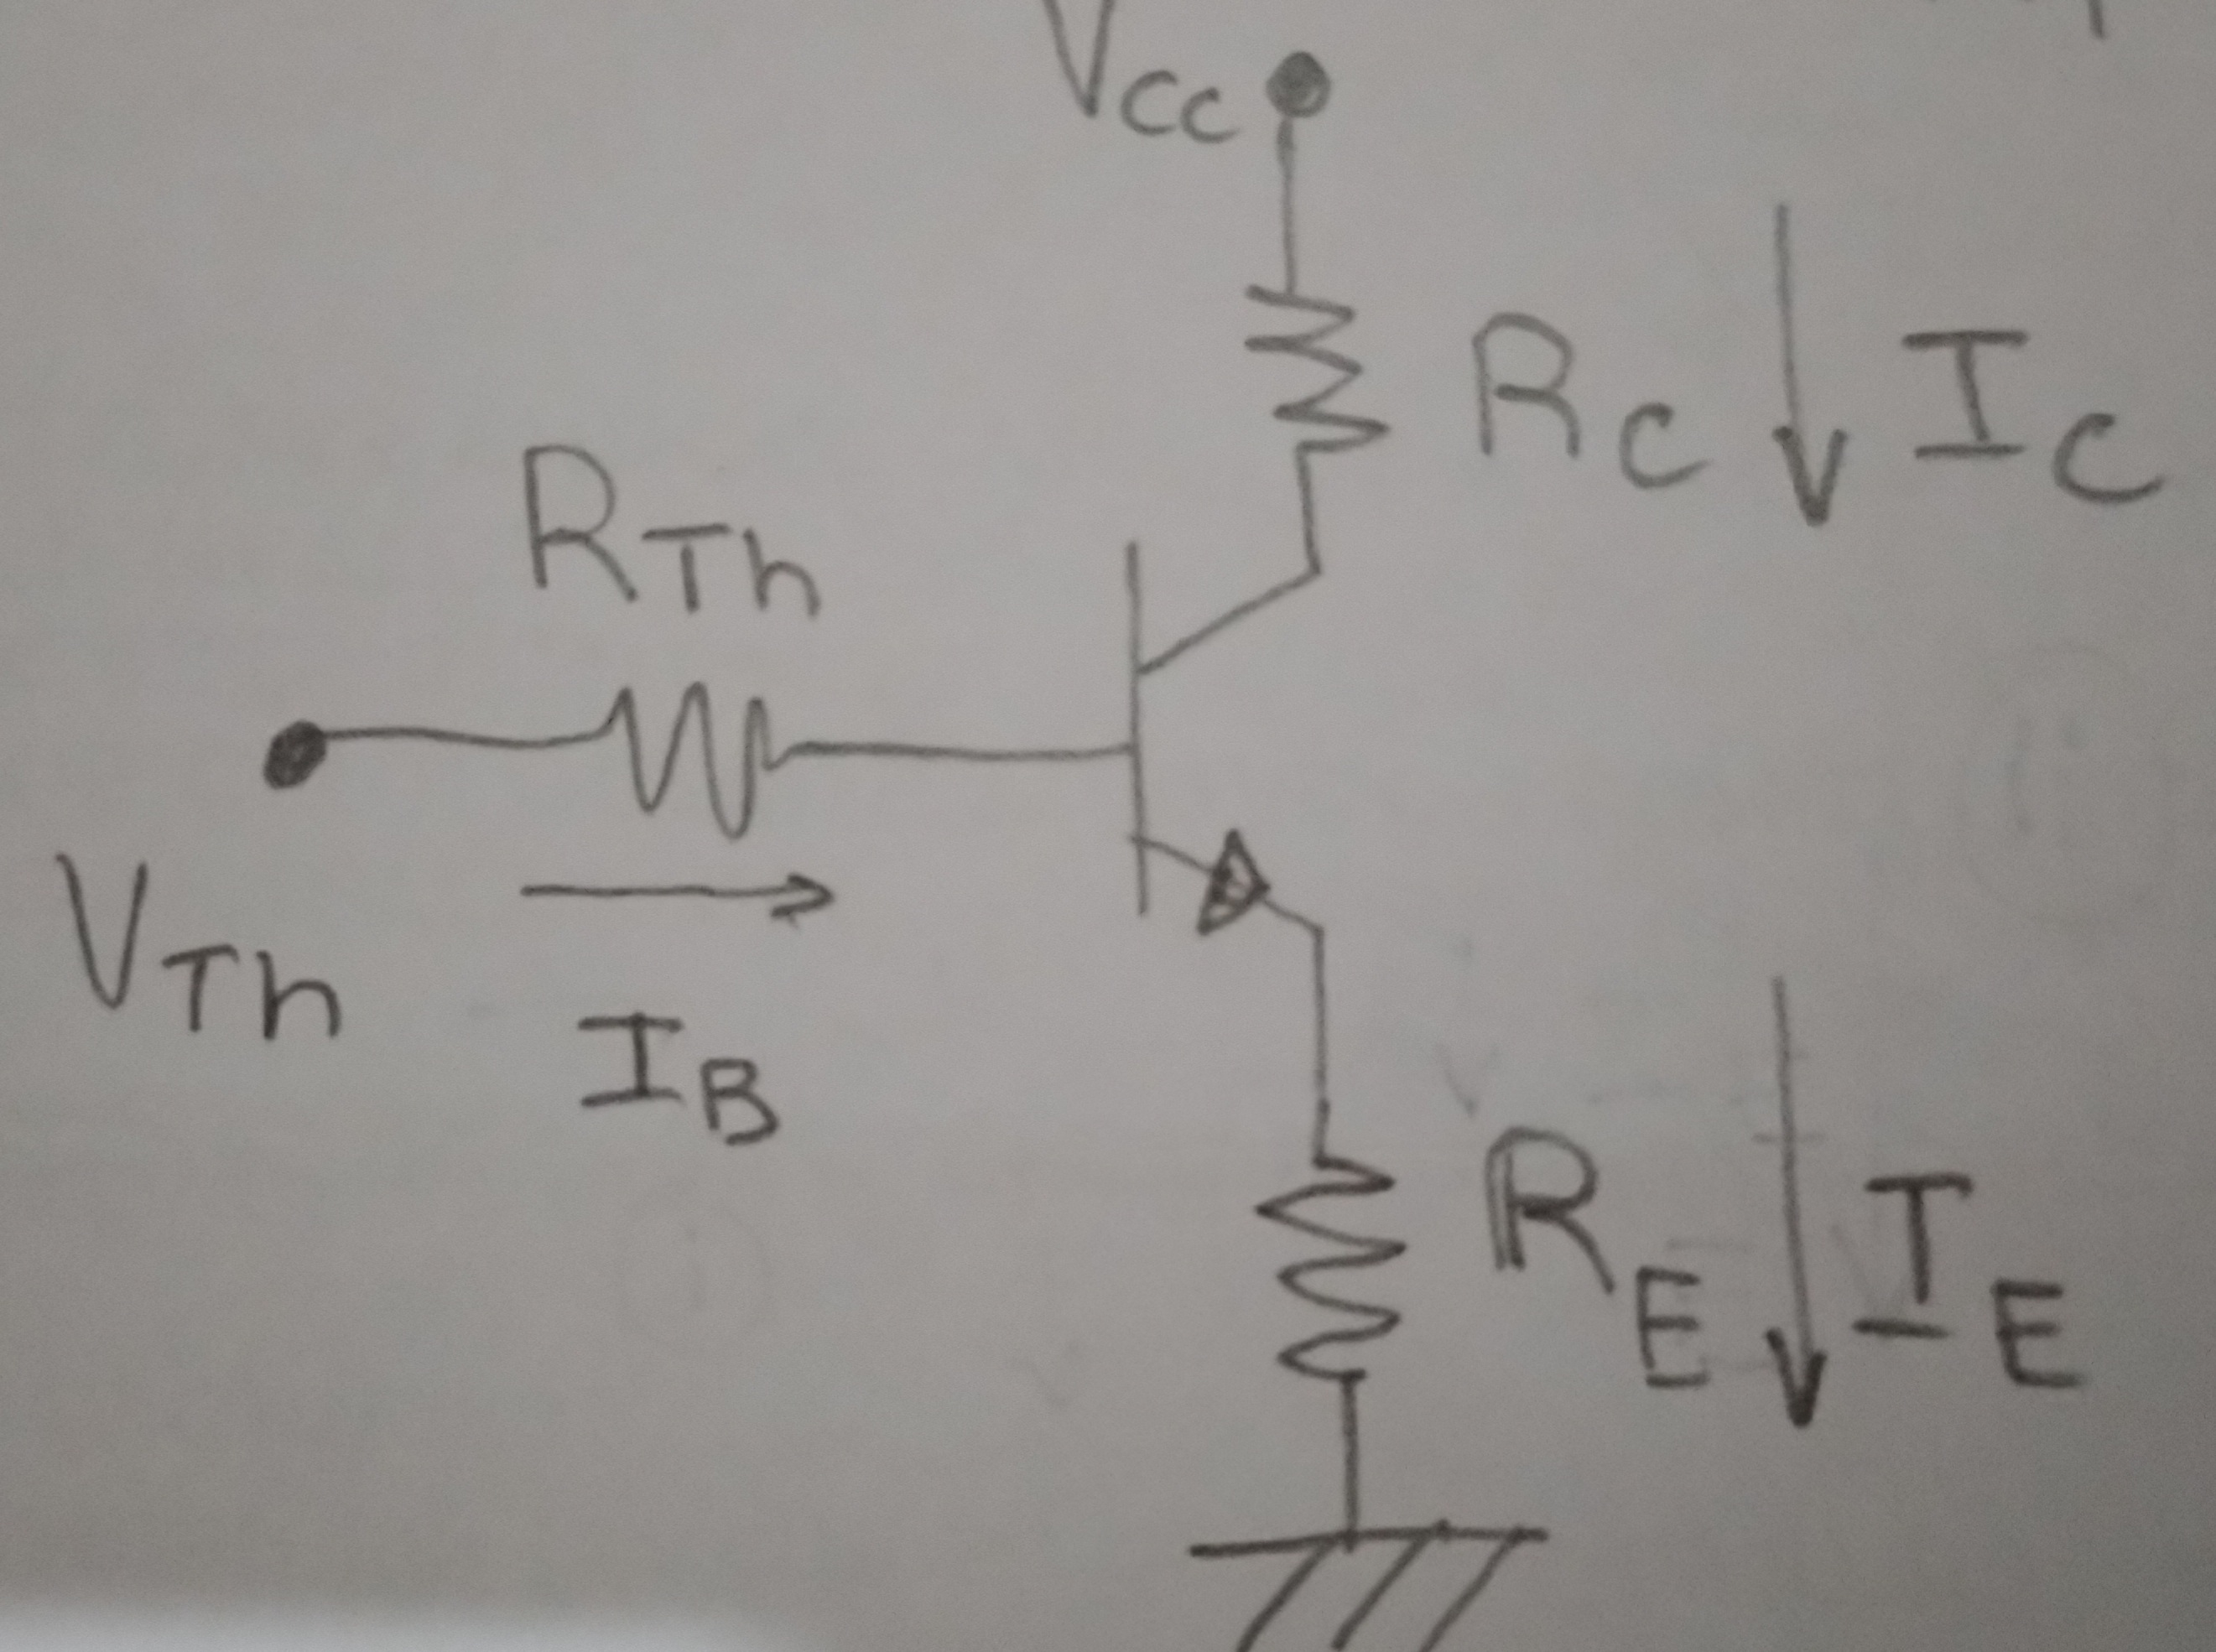
\includegraphics[height=4cm\textwidth]{thqestatico.jpg} \par
        \caption{Circuito de operación estática simplificado Thevelin}
        \label{fig:2}
    \end{figure}

    aplicando ley de tensiones de Kirchoff

    $$R_{Th}I_B + V_{BE} + R_EI_E = V_{Th}$$

    si $I_E = (\beta + 1)I_B$, entonces

    $$R_{Th}I_B + V_{BE} + R_E(\beta + 1)I_B = V_{Th}$$

    $$I_B = {V_{Th} - V_{BE} \over R_{Th} + R_E(\beta + 1)}$$

    Sustituyendo valores

    $$I_B = {3.4V - 0.7V \over 25.8k\Omega + 200\Omega(150 + 1)} = 0.048mA$$

    sabiendo que $I_C = \beta I_B$

    $$I_C = 150(0.048mA) = 7.23mA$$

    aplicando ley de tensiones de Kirchoff a la otra malla

    $$R_{C}I_C + V_{CE} + R_EI_E = V_{CC}$$

    $$V_{CE} = V_{CC} - R_{C}I_C - R_E(\beta + 1)I_B$$

    sustituyendo

    $$V_{CE} = 12V - 510\Omega (7.23mA) - 200\Omega (150 + 1) 0.048mA = 6.86V$$

    Punto de operacion

    \begin{split}
        Q & : (V_{CE}, I_C) \\
        Q & : (6.86V, 7.23mA)
    \end{split}

    Por lo tanto se puede decir que está trabajando en la zona activa y en consecuencia puede amplificar una señal.

    Utilizando el modelo de parametros híbridos de la Figura \ref{fig:h1} sin tomar en cuenta RL ni CE

    \begin{figure}[h!]
        \centering
        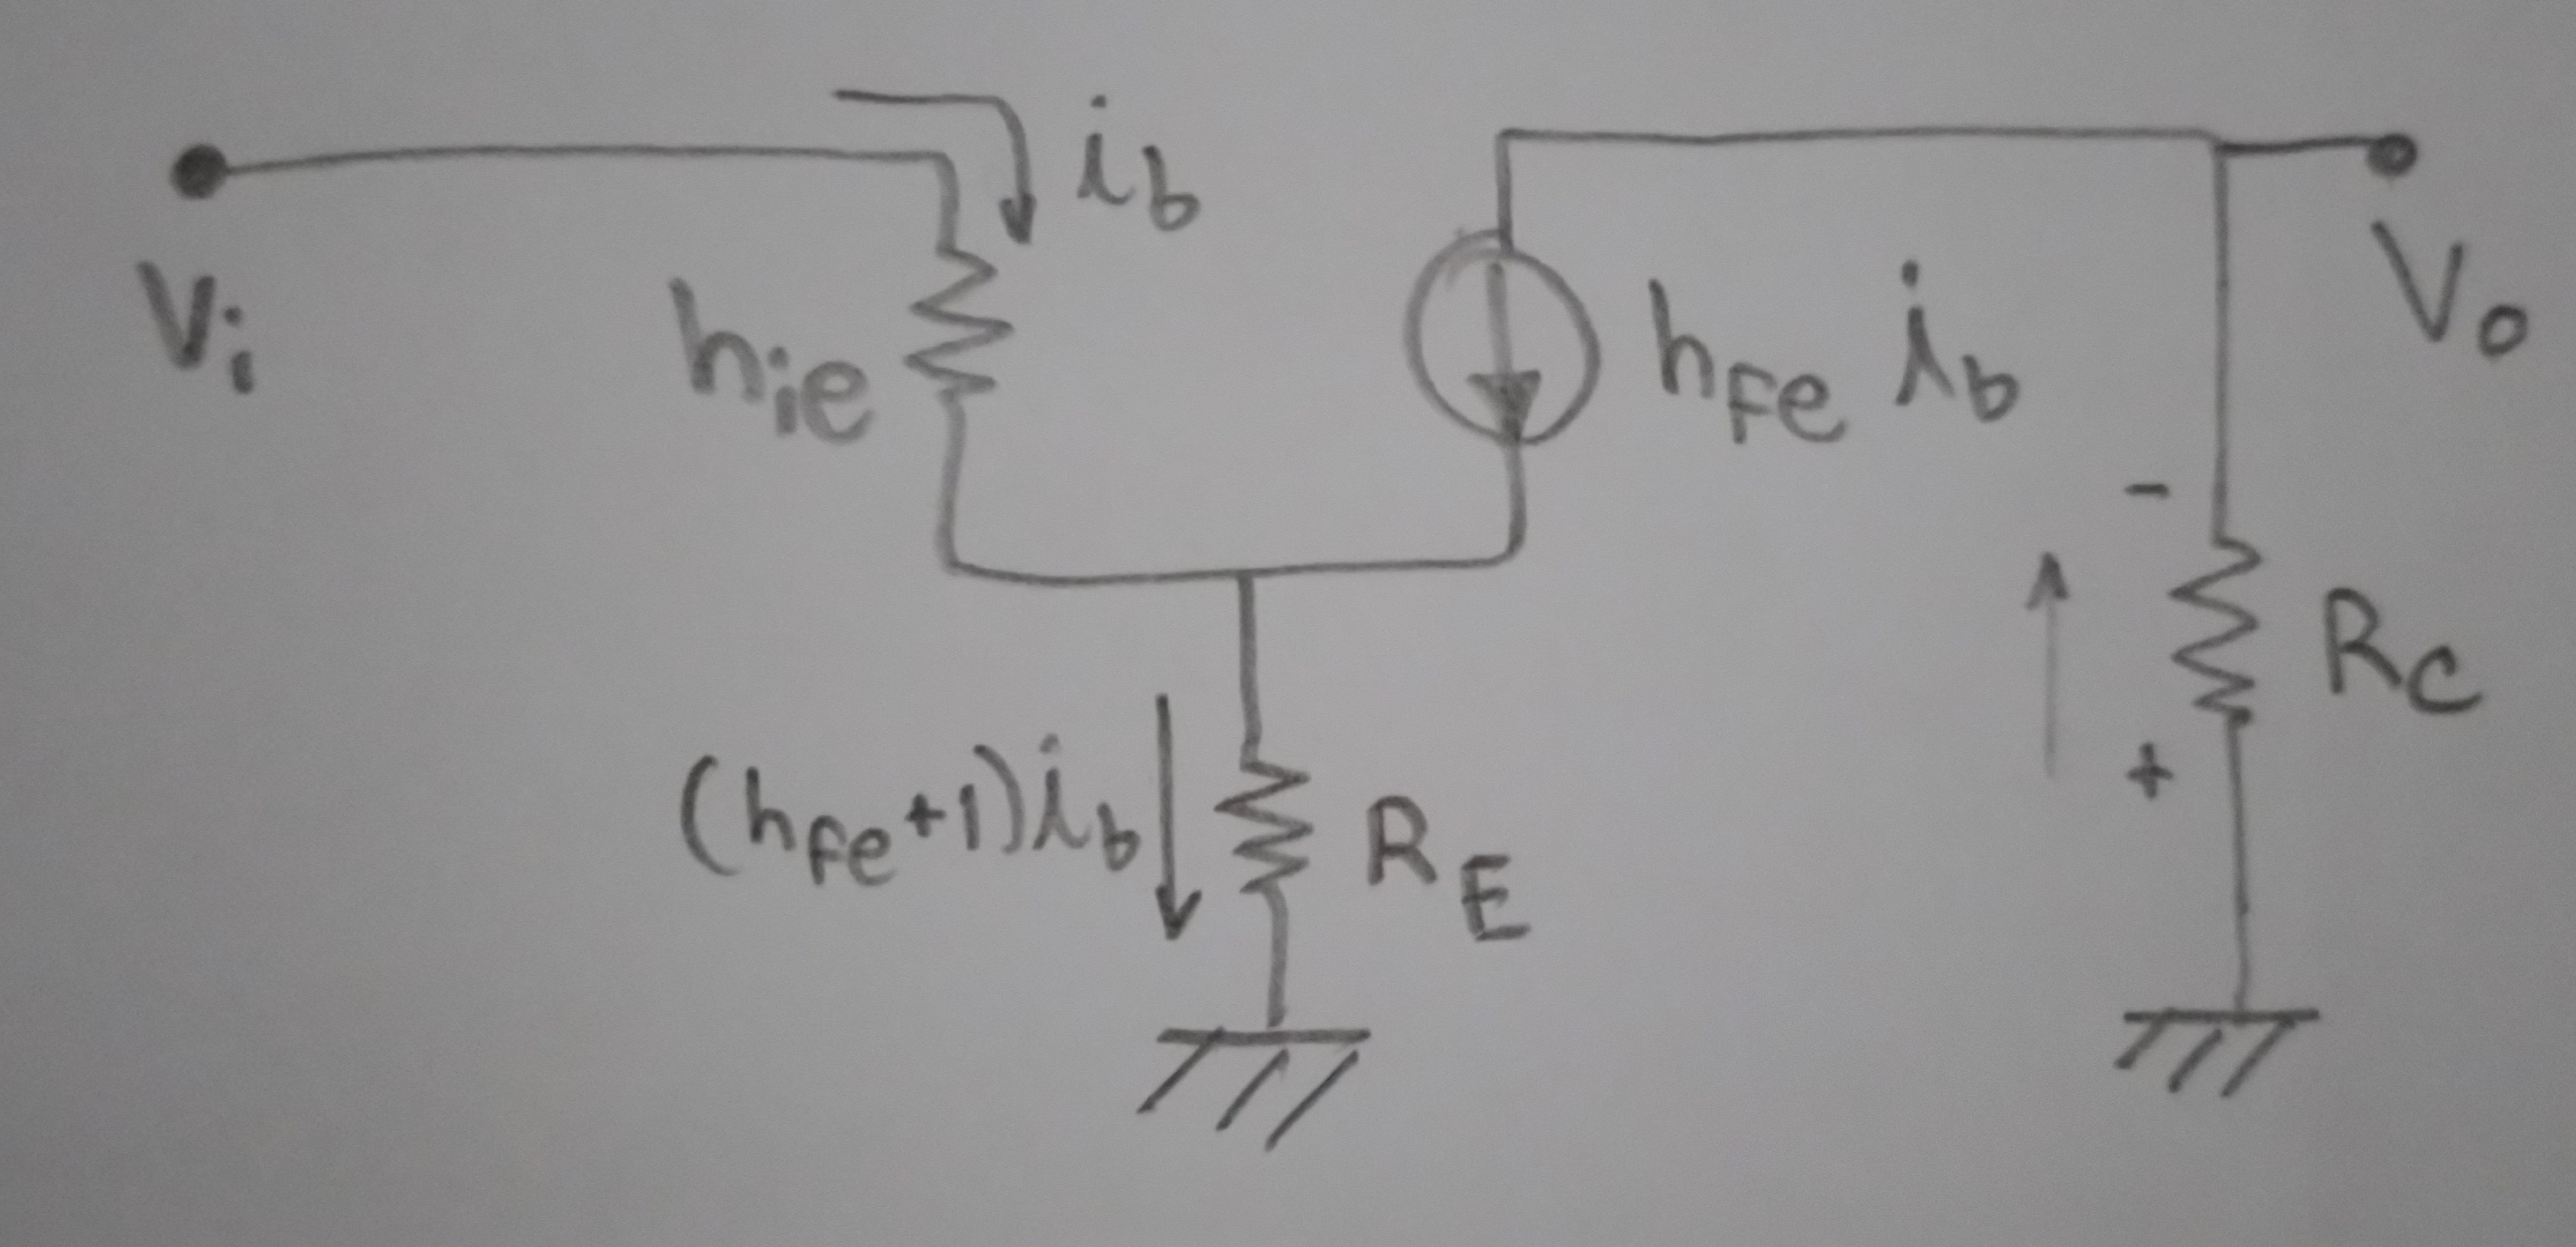
\includegraphics[height=4cm\textwidth]{h1.jpg} \par
        \caption{Modelo de parametros híbridos sin RL ni CE}
        \label{fig:h1}
    \end{figure}

    Se puede apreciar en la figura \ref{fig:h1} que $R_1$ y $R_2$ actúa como un corto a tierra debido al capacitor que se encuentra en la entrada, donde se asume una señal media.

    Sabiendo que

    \begin{equation}
        A_V = {V_o \ over V_i}
        \label{eq1}
    \end{equation}

    Además si

    $$V_i = i_bh_{ie} + (h_{fe}+1)i_bR_E = i_b(h_{ie} + (h_{fe}+1)R_E)$$

    $$V_o = -h_{fe}i_bR_C$$

    Sustituyendo lo anterior en \ref{eq1}

    \setcounter{equation}{1}
    \begin{equation}
        A_V = -\frac{h_{fe}R_C}{h_{ie} + (h_{fe}+1)R_E}
        \label{eq2}
    \end{equation}

    Reemplazando parametros

    $$A_V = -\frac{-(175)(510\Omega)}{5K\Omega + (175+1)(200\Omega)} = -2.22 V/V$$

    Para calcular las impedancias no se toma en cuenta el condensador acoplado, entonces:

    \setcounter{equation}{1}
    \begin{equation}
        Z_i = R_{Th}||Z_1
        \label{eq3}
    \end{equation}

    si

    $R_{Th} = R_1||R_2 = 25.8K\Omega$

    \begin{split}
        Z_1 & = {V_i \over i_b} = \frac{i_b(h_{ie} + (h_{fe}+1)R_E)}{i_b} = h_{ie} + (h_{fe}+1)R_E \\
        Z_1 & = 5K\Omega + (175+1)(200\Omega) = 40.2K\Omega
    \end{split}

    En \ref{eq3}

    $$Z_i = 25.8K\Omega||40.2K\Omega = 15.7K\Omega$$

    Además

    $$Z_o = R_C = 510\Omega$$
    
    Utilizando el modelo de parametros híbridos de la Figura \ref{fig:h2} tomando en cuenta solamente RL

    \begin{figure}[h!]
        \centering
        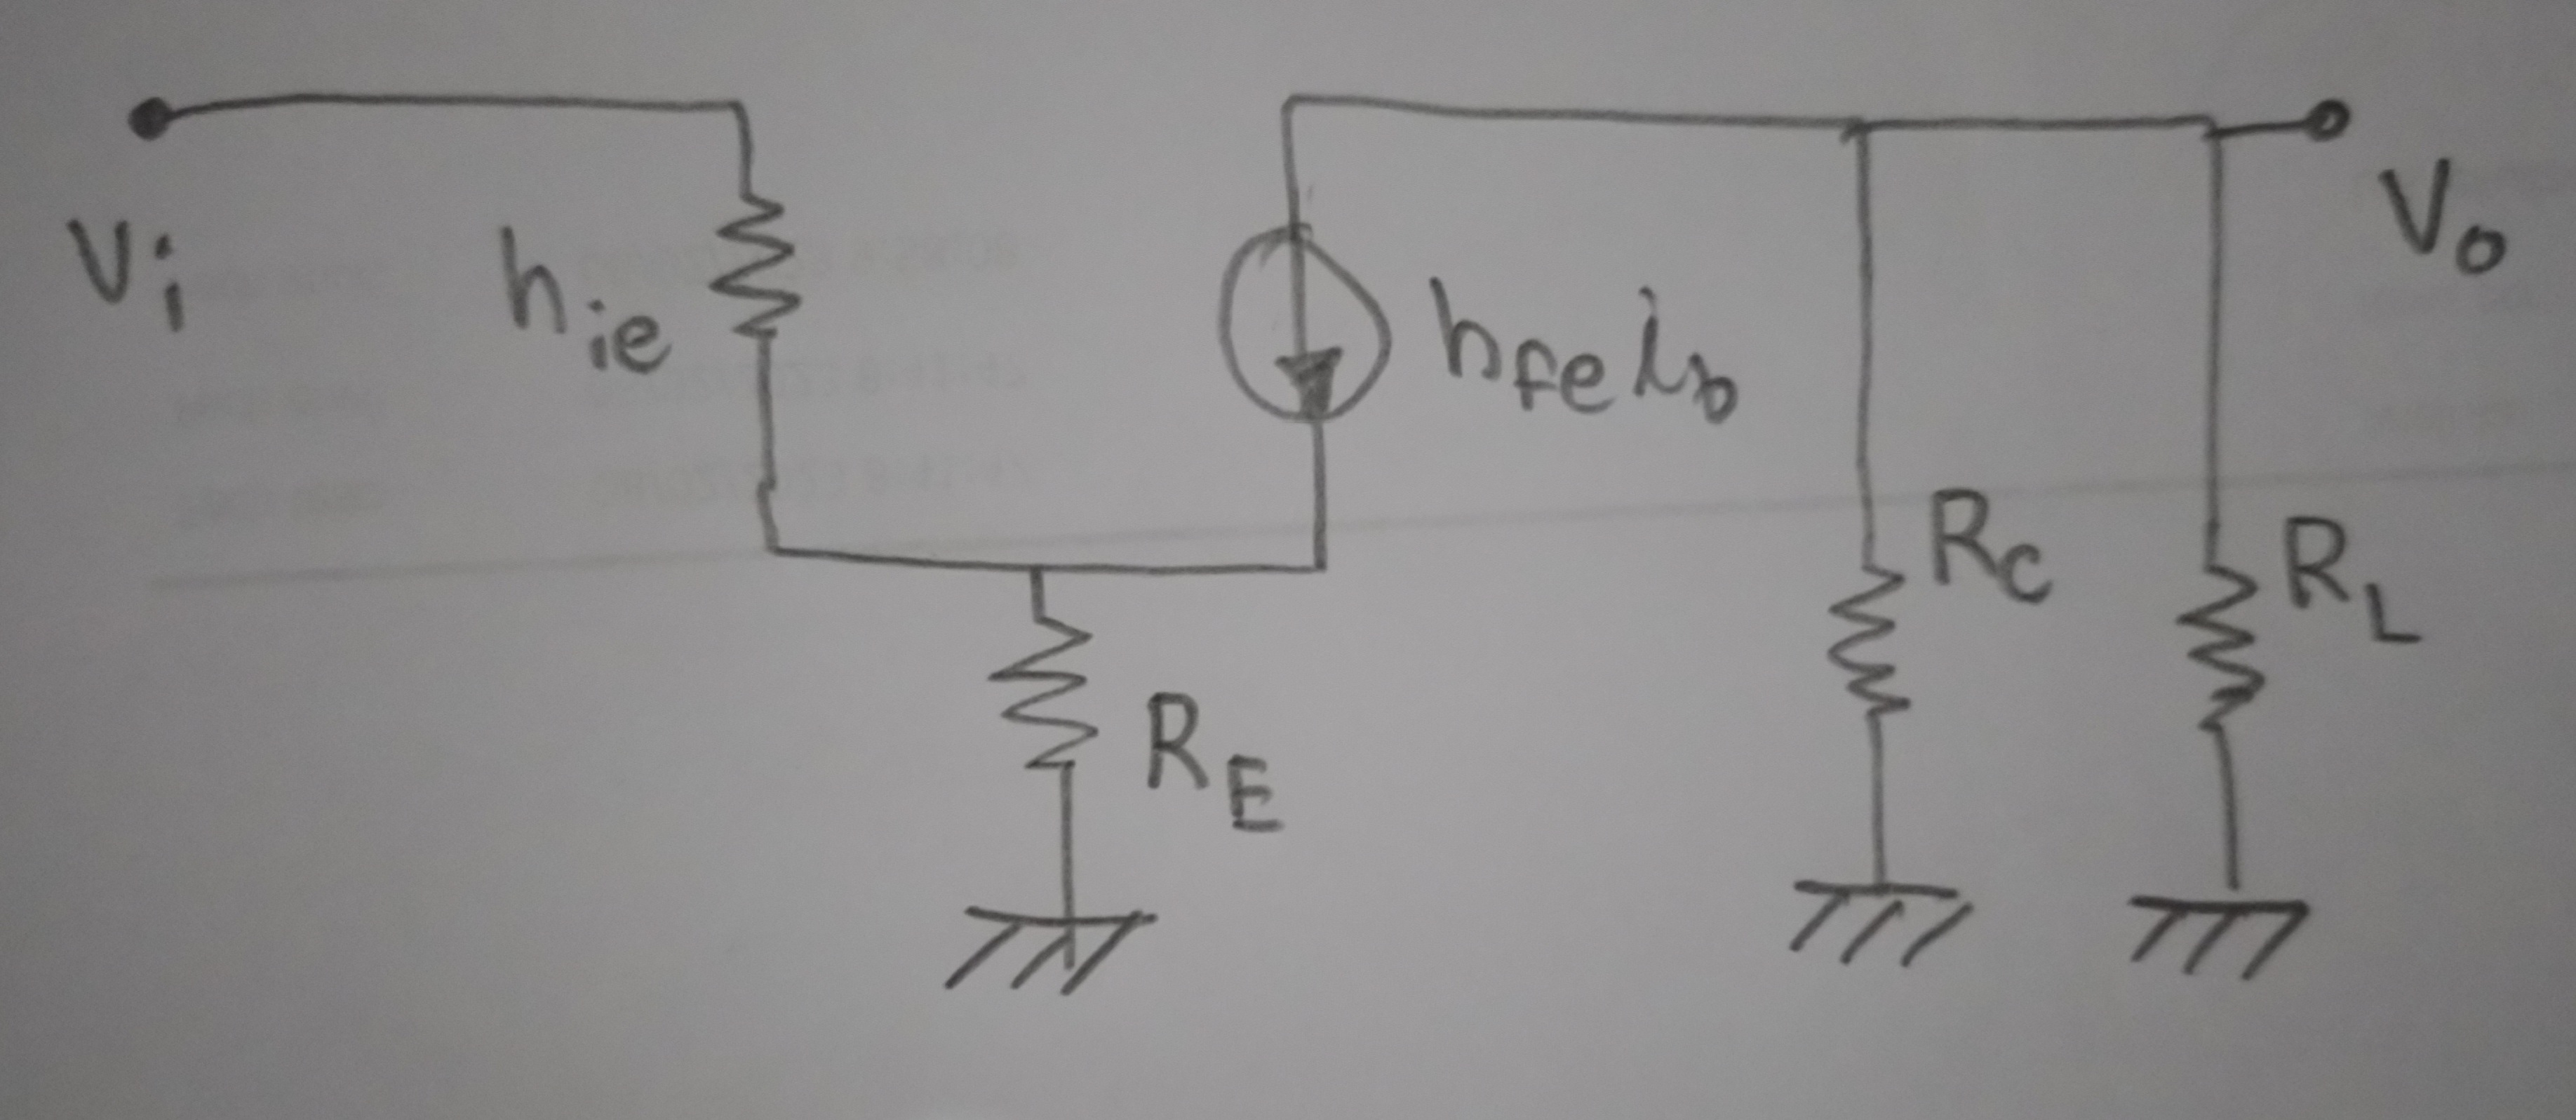
\includegraphics[height=4cm\textwidth]{h2.jpg} \par
        \caption{Modelo de parametros híbridos con RL}
        \label{fig:h2}
    \end{figure}

    Adaptando la ecuación \ref{eq2} a

    \setcounter{equation}{1}
    \begin{equation}
        A_V = -\frac{h_{fe}R'_C}{h_{ie} + (h_{fe}+1)R_E}
        \label{eq4}
    \end{equation}

    donde
    
    \begin{split}
        R'_C & = R_C||R_L = \frac{R_CR_L}{R_C + R_L} \\
        R'_C & = \frac{(510\Omega)(10K\Omega)}{510\Omega + 10K\Omega} = 485\Omega
    \end{split}

    En \ref{eq4}

    $$A_V = -\frac{-(175)(485\Omega)}{5K\Omega + (175+1)(200\Omega)} = -2.11 V/V$$

    Ya que la entrada no se ve afectada por RL, la impedancia de entrada $Z_i$ nom sufre modificación

    $$Z_i = 15.7K\Omega$$

    Para la impedancia de salida

    $$Z_o = R'_C = 485\Omega$$

    Utilizando el modelo de parametros híbridos de la Figura \ref{fig:h2} tomando en cuenta solamente CE

    \begin{figure}[h!]
        \centering
        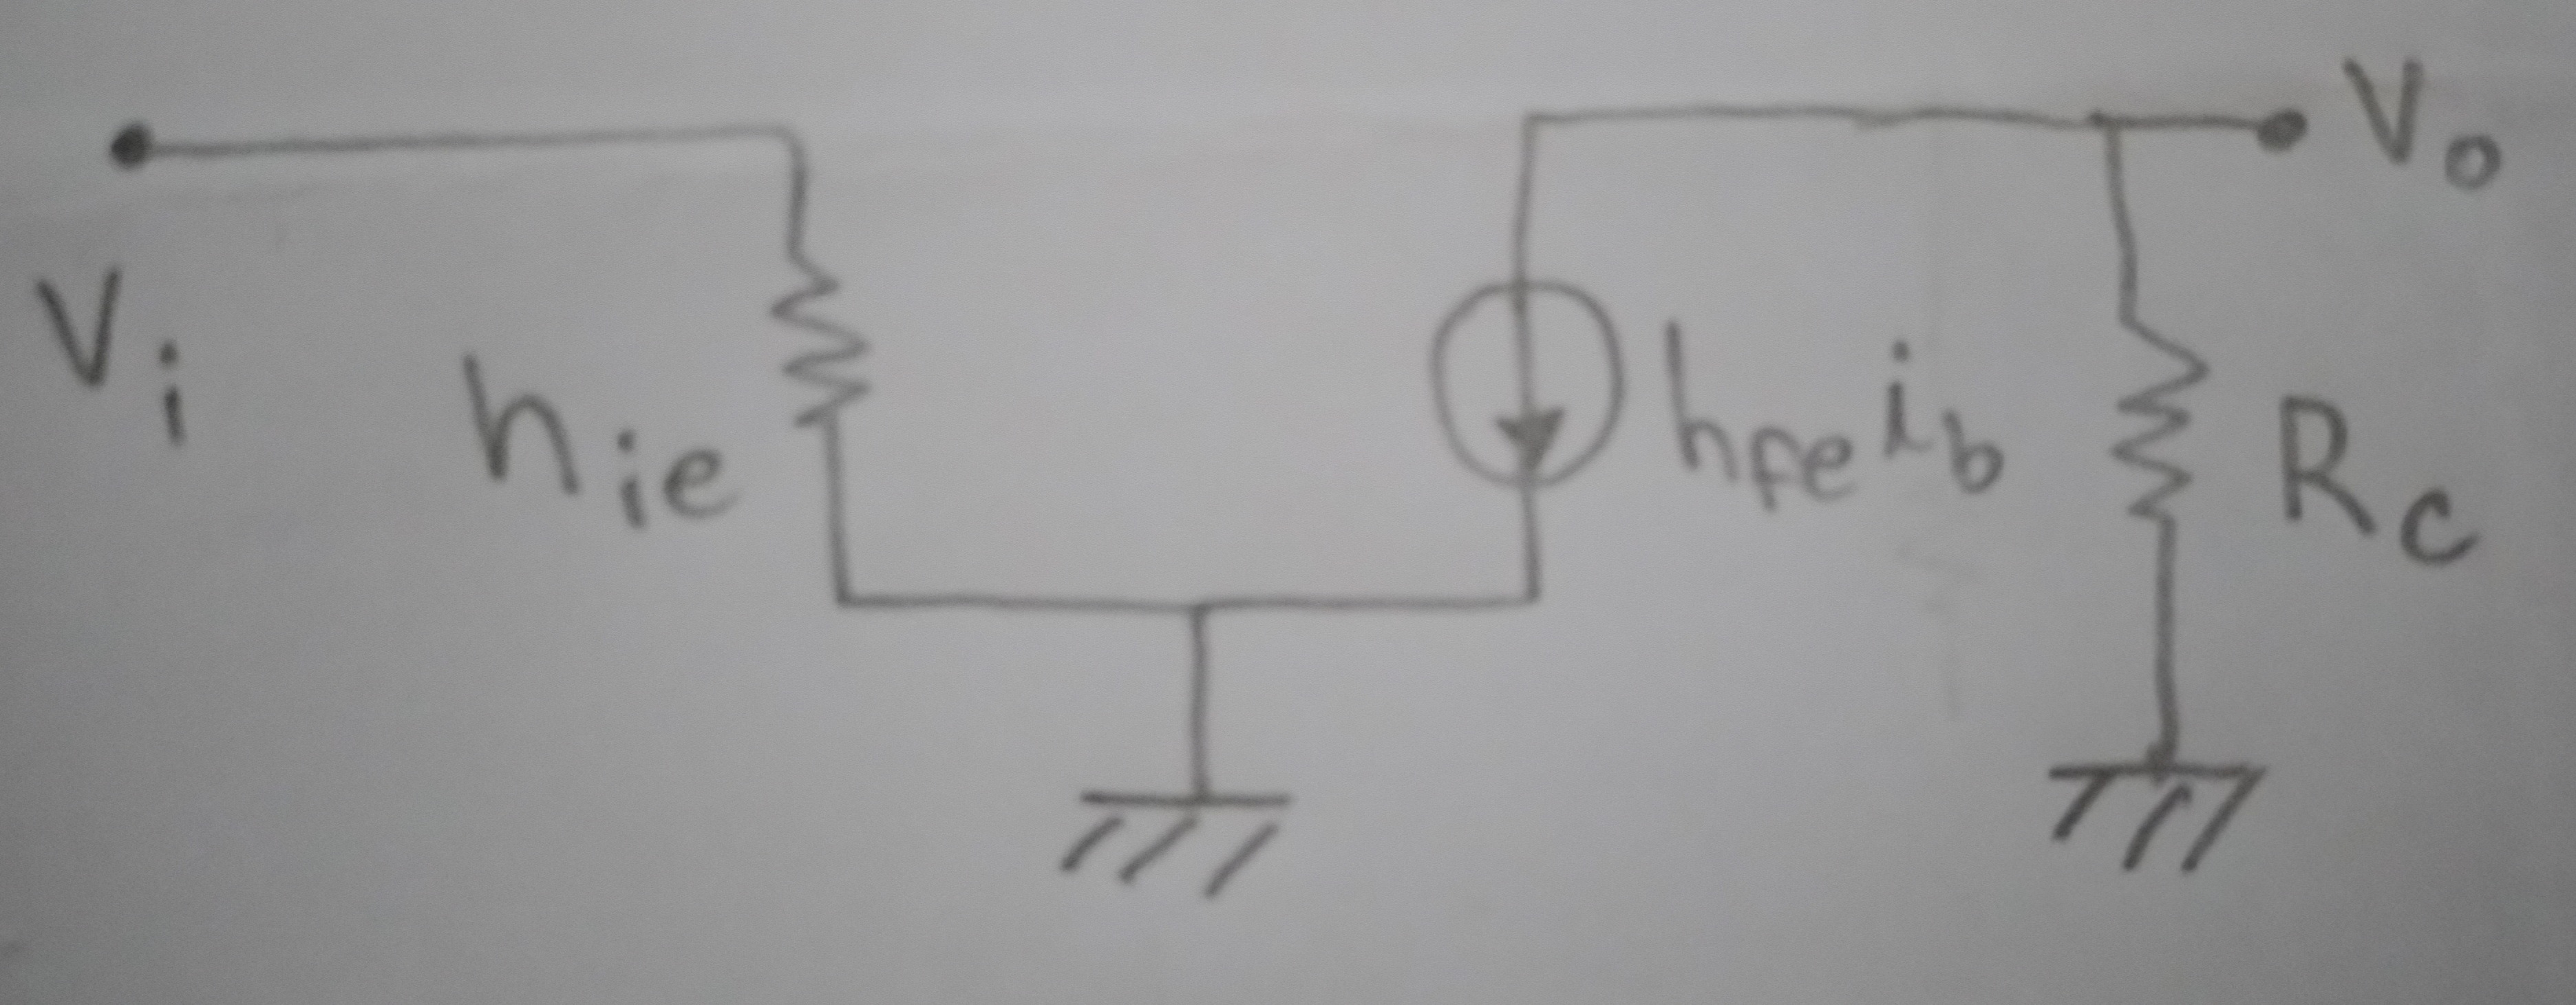
\includegraphics[height=4cm\textwidth]{h3.jpg} \par
        \caption{Modelo de parametros híbridos con CE}
        \label{fig:h3}
    \end{figure}

    Sabiendo que

    $V_i = h_{ie}i_b$

    $V_o = -h_{fe}i_bR_C$

    Reemplazando en \ref{eq1} se demuestra que

    \setcounter{equation}{1}
    \begin{equation}
        A_V = -{h_{fe}R_C \over h_{ie}}
        \label{eq5}
    \end{equation}

    sustituyendo parametros

    $$A_V = -{(175)(510\Omega) \over 5K\Omega} = -17.85 V/V$$

    Para el cálculo de la impedancia de entrada se hace uso de \ref{eq3}, donde

    \begin{split}
        Z_1 & = {V_i \over i_b} = \frac{i_bh_{ie}}{i_b} = h_{ie} \\
        Z_1 & = 5K\Omega
    \end{split}

    sustituyendo en \ref{eq3}

    $$Z_i = R_{Th}||Z_1 = 25.8K\Omega||5K\Omega = 4.2K\Omega$$

    Además

    $$Z_o = R_C = 510\Omega$$

    \begin{figure}[h!]
        \centering
        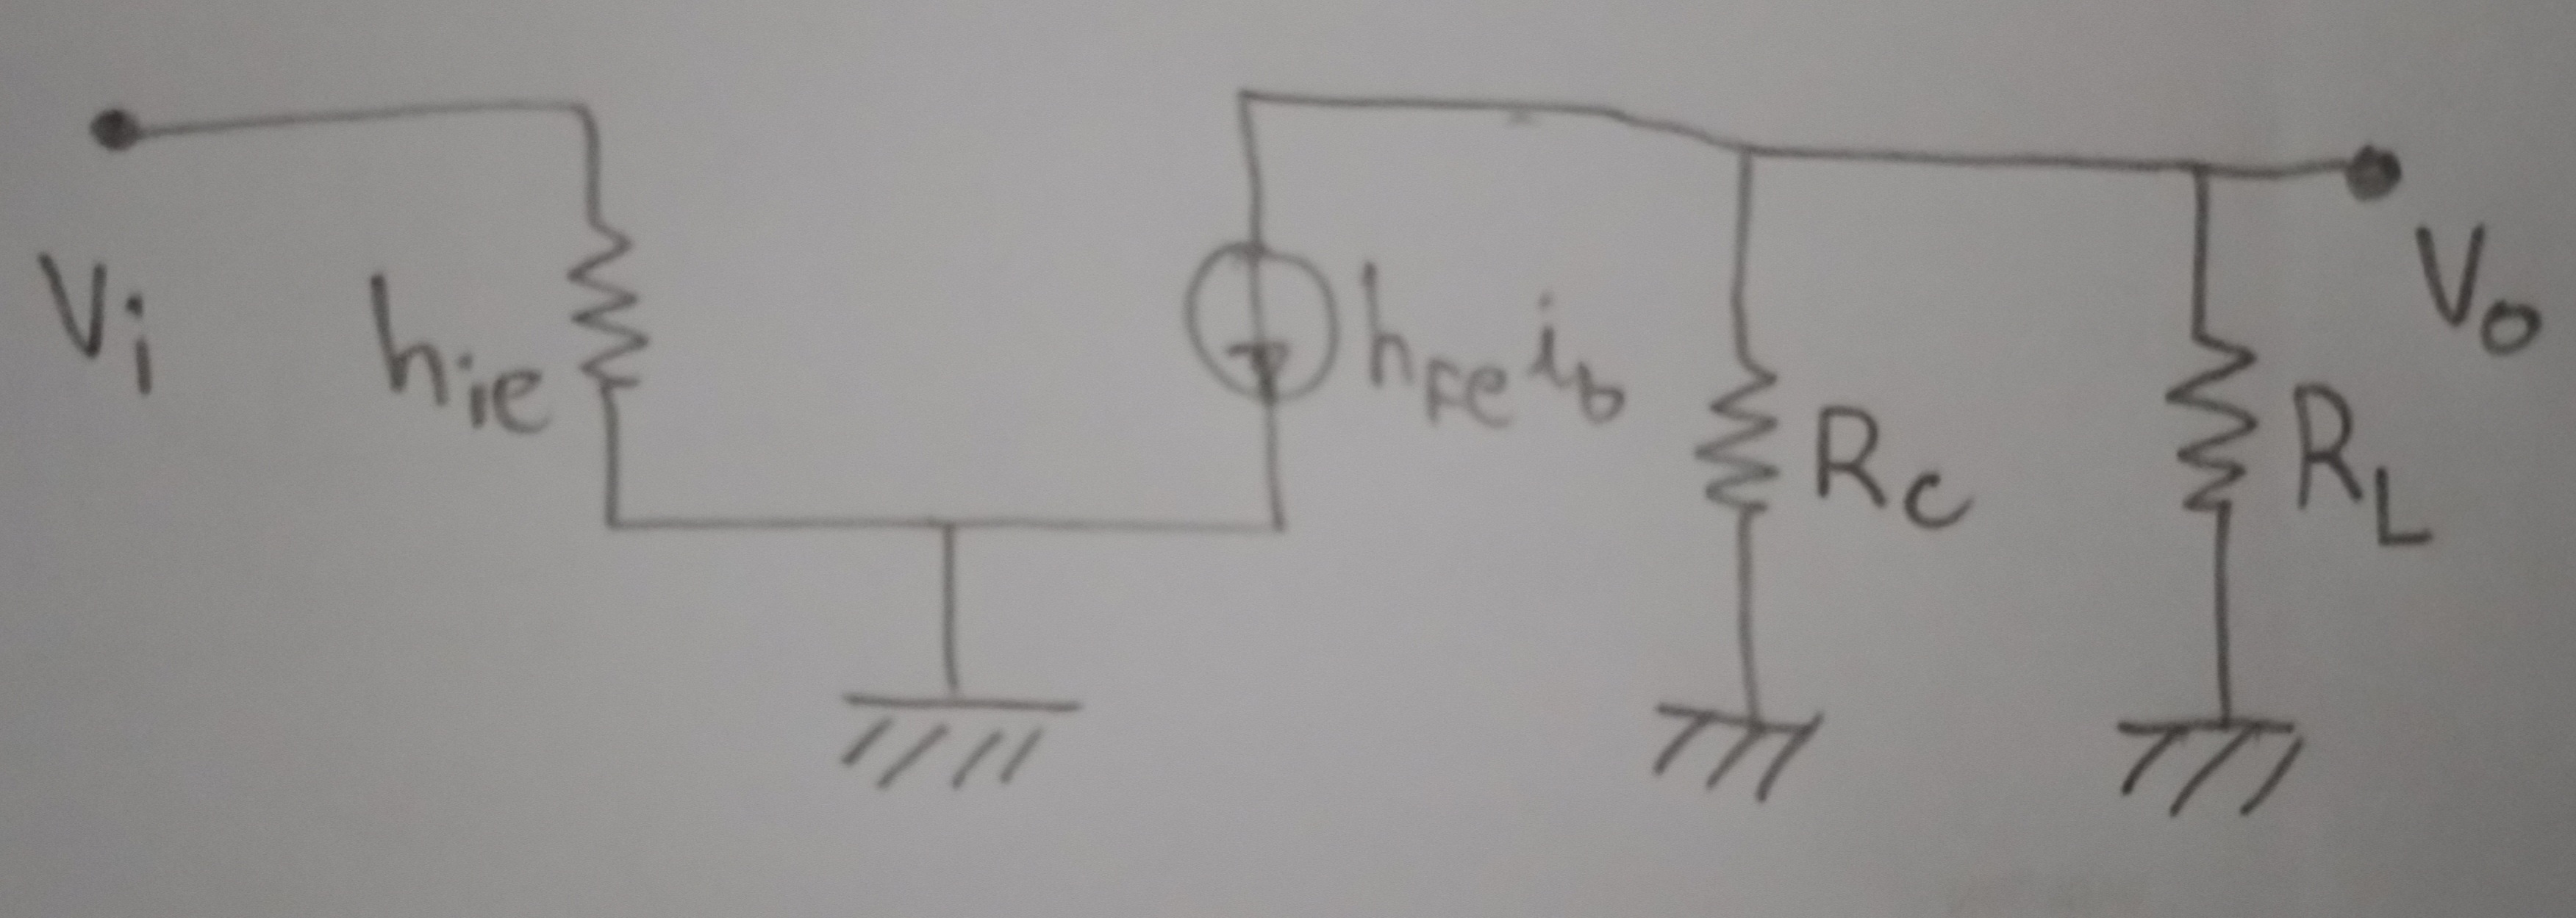
\includegraphics[height=4cm\textwidth]{h4.jpg} \par
        \caption{Modelo de parametros híbridos con RL y CE}
        \label{fig:h4}
    \end{figure}

    Adaptando \ref{eq5}

    \setcounter{equation}{1}
    \begin{equation}
        A_V = -{h_{fe}R'_C \over h_{ie}}
        \label{eq6}
    \end{equation}

    donde $R'_C = 485\Omega$, ya calculado antes

    entonces en \ref{eq6}

    $$A_V = -{(175)(485\Omega) \over 5K\Omega} = -16.98V/V$$

    La impedancia de entrada $Z_i$ no cambia con respecto a la calculada en el caso anterior

    $$Z_i = 4.2K\Omega$$

    Además

    $$Z_o = R'_C = 485\Omega$$

    \newpage

    \section{Materiales e Instrumentos}

    %hay que realizar tablas

    \begin{itemize}
        \item Transistor npn PN2222A
        \item Resistencia de carbon de $91k\Omega$  serie del $5\%$ y potencia de $1/4$ W.
        \item Resistencia de carbon de $510\Omega$  serie del $5\%$ y potencia de $1/4$ W.
        \item Resistencia de carbon de $200\Omega$  serie del $5\%$ y potencia de $1/4$ W.
        \item Resistencia de carbon de $36k\Omega$  serie del $5\%$ y potencia de $1/4$ W.
        \item Resistencia de carbon de $10k\Omega$  serie del $5\%$ y potencia de $1/4$ W.
        \item Condensadores electrolíticos de $10\mu F$, $16 V$.
    \end{itemize}

\end{document}